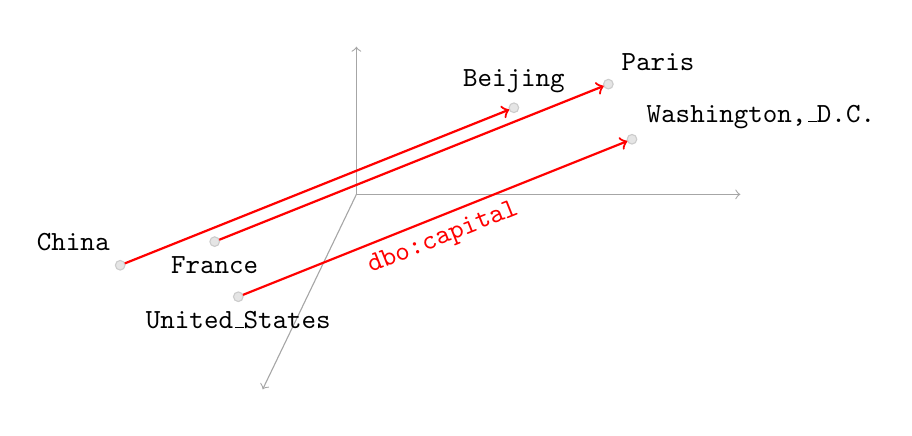
\begin{tikzpicture}
[   cnode/.style={draw=gray!40,fill=gray!20,text width=1mm, scale=0.3, circle},
    rnode/.style={draw=black,fill=#1,minimum width=6mm, minimum height=5mm, rectangle},
    rline/.style={red,thick, ->}
]
    
    \def\rx{5};
    \def\ry{2};
    
    \def\ox{0.5*\rx};
    \def\oy{0.5*\ry};
    \node (origin) at (\ox, \oy) {};
    \node (x) at (\ox + 1 * \rx, \oy) {};
    \node (y) at (\ox - 0.25*\rx, \oy-1.3*\ry) {};
    \node (z) at (\ox, \oy+2) {};
    
    \draw[gray!70, ->] (origin.center) -- (x);
    \draw[gray!70, ->] (origin.center) -- (y);
    \draw[gray!70, ->] (origin.center) -- (z);
    
    \node[cnode, label={100:\texttt{China}}] (a1) at (-0.5, 0.1) {};
    \node[cnode, label={270:\texttt{United\_States}}] (a2) at (1, -0.3)   {};
    \node[cnode, label={270:\texttt{France}}] (a3) at (0.7, 0.4)  {};
    
    \node[cnode, label={\texttt{Beijing}}] (b1) at (-0.5+\rx, 0.1+\ry)  {};
    \node[cnode, label={10:\texttt{Washington,\_D.C.}}] (b2) at (1+\rx, -0.3+\ry) {};
    \node[cnode, label={45:\texttt{Paris}}] (b3) at (0.7+\rx, 0.4+\ry)  {};
    
    \draw[rline] (a1) -- (b1);
    \draw[rline] (a2) -- node[below, sloped]{\texttt{dbo:capital}} (b2);
    \draw[rline] (a3) -- (b3);
    
    % \draw[->,blue,thick] (0,0) -- node[above, sloped]{$\mathbf{h}$} % (1, 1.8);
    % \draw[->,red, thick] (0,0) -- node[above, sloped]{$\mathbf{t}$} % (3, 1.2);
    % \draw[->] (1,1.8) -- node[above, sloped]{$\mathbf{r}$} (2.9, % 1.25);
    
    % \draw[->] (0,0) -- (4,0);
    % \draw[->] (0,0) -- (-0.5, -0.75);
    % \draw[->] (0,0) -- (0,2);
    
    % \node at (2, -1.5) {$(h, r, t) \in \mathcal{KG} \iff \mathbf{h} + \mathbf{r} \approx \mathbf{t} $}
\end{tikzpicture}